%
\againframe{plan}
%
\begin{frame}{\(V(x)\): Finite barrier potential}
		%
	\begin{columns}
		%
		\begin{column}{0.6\textwidth}
			\[
			V(x) =  
			\left\{
			\begin{array}{ll}
				V_0	&	-\frac{a}{2} < x < \frac{a}{2}	\\
				0		&	\text{otherwise}	\\
			\end{array}
			\right.
			\]
		\end{column}
		%
		\begin{column}{0.38\textwidth}
			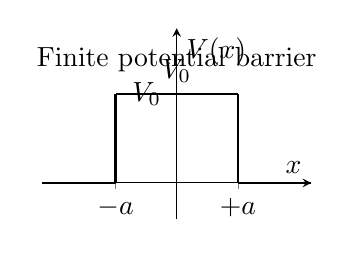
\begin{tikzpicture}
				\def\w{5.0cm}   % width of each plot
				\def\h{4.0cm}   % height of each plot
				% ---------- 3) Finite potential barrier ----------
				\begin{axis}[
					at={(12.4cm,0)}, anchor=south west,
					width=\w,height=\h,
					axis lines=middle,
					xmin=-2.2, xmax=2.2,
					ymin=-1.2, ymax=5.2,
					xtick={-1,1},
					xticklabels={\( -a\), \( +a\)},
					ytick={0,3},
					yticklabels={0,$V_0$},
					xlabel={$x$},
					ylabel={$V(x)$},
					title={Finite potential barrier},
					every axis title/.style={at={(0.5,0.95)},anchor=north},
					clip=false
					]
					% left and right baseline V = 0
					\addplot[thick,domain=-2.2:-1,samples=2] ({x},{0});
					\addplot[thick,domain=1:2.2,samples=2] ({x},{0});
					% barrier region: positive finite height (e.g. 3)
					\addplot[thick] coordinates {(-1,3) (1,3)};
					% vertical steps at boundaries
					\addplot[thick] coordinates {(-1,0) (-1,3)};
					\addplot[thick] coordinates {(1,0) (1,3)};
					% label
					\node[anchor=south] at (axis cs:0,3.05) {\(\displaystyle V_0\)};
				\end{axis}
			\end{tikzpicture}
		\end{column}
	\end{columns}
	\hrule
\end{frame}
%
\begin{frame}{Quantum tunnelling: probability}
	\begin{guesstimate}{Tunnelling probability}
		\begin{enumerate}
			\item Effective mass of electron in \ce{GaAs} is \(0.067\, m_0\).
			\item Rectangular potential barrier of height \(V_0 = \SI{0.8}{\electron\volt}\) and width \SI{15}{\angstrom}.
			\item The kinetic energy of electron is \SI{0.20}{\electron\volt}
		\end{enumerate}
		Repeat the steps for electron in \ce{Si} with effective mass of \(1.08\, m_0\).
	\end{guesstimate}
\end{frame}